\chapter{Definitions}

\section{Module}
On module in the terminology of Plantage is just a rectangular shape. From that point of view every circuit element can be viewed as module, transistors, capacitors, and son on. It can contain pins, but for the placement only the width and height are important. The actual dimensions are stored the variant for the module. Every module can have various different variants, for example with the same electrical behaviour, but different numbers of gates [\ref{fig:modules_with_different_gate_number}].

\begin{figure}
	\centering
	\setlength{\unitlength}{0.282222229121mm}
\begin{picture}(520.0, 200.0)(0, -200.0)
  \put(0,-200.0){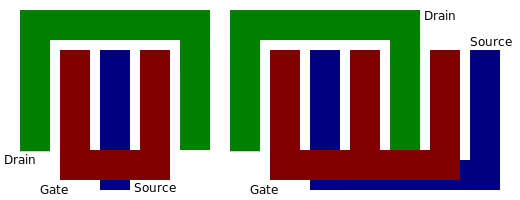
\includegraphics[height=56.4444458242mm, width=146.755559143mm]{FIG/modules_with_different_gate_number.svg.pdf}}
  \put(40.0,-194.00002){\makebox(0,0)[l]{\smash{Gate}}}
  \put(4.0,-164.00002){\makebox(0,0)[l]{\smash{Drain}}}
  \put(134.0,-192.00002){\makebox(0,0)[l]{\smash{Source}}}
  \put(250.0,-194.00002){\makebox(0,0)[l]{\smash{Gate}}}
  \put(424.0,-20.0){\makebox(0,0)[l]{\smash{Drain}}}
  \put(470.0,-46.0){\makebox(0,0)[l]{\smash{Source}}}
\end{picture}
	\caption{the same MOSFET with two different numbers of gates}
	\label{fig:modules_with_different_gate_number}
\end{figure}

Also a module typically has some pins, which are named themselves and have a net name, which they belong to. One pin can have some contact areas, but must have at least one. Every contact area is only a rectangular shape, which has a height and width and is positioned relative to the module position.

\section{Group}
In Plantage there are two different types of groups. One type contains only groups and the other one only modules [\ref{fig:group_of_modules}]. At the moment it is not supported to mix modules and groups in one group. This is important, because slightly different algorithms must be applied for every type of group.

\begin{figure}
	\centering
	\subfloat[group of single modules]{
\includegraphics[scale=0.5]{FIG/group_of_modules.png}}
	\subfloat[group of two groups]{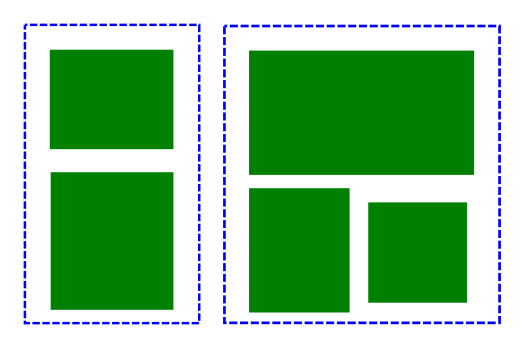
\includegraphics[scale=0.5]{FIG/group_of_groups.png}}
	\caption{groups arrange modules and groups together}
\end{figure}

\section{Shapefunction}
A shape function is basically a list of possible layouts for a given circuit. This list is called shapefunction [\ref{fig:shapefunction}], because the minimum possible area for these placements is a hyperbolic function and the placements are located near to this so called pareto front.

\begin{figure}
	\centering
	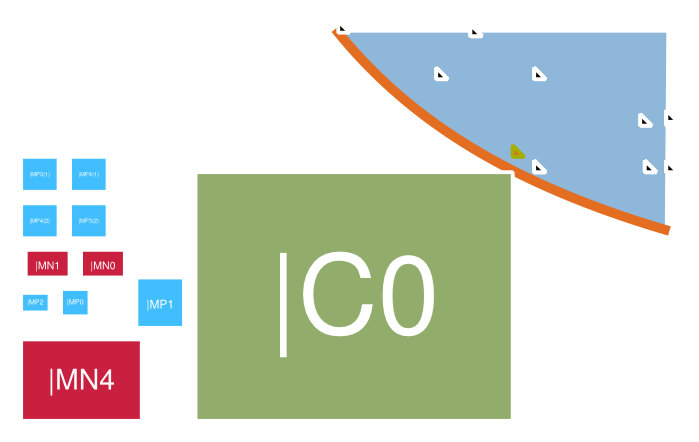
\includegraphics[scale=1.8]{FIG/shapefunction.png}
	\caption{shapefunction with possible placements for a miller amplifier}
	\label{fig:shapefunction}
\end{figure}

\subsection{Shape}
A shape is the layout for a certain couple of modules. On the one hand it is used for the layout of the whole circuit, but on the other hand also for the layout of only circuit parts.

\section{Constraints}
In the design of analog circuits a bunch of constraints have to be met. The mainly consider, that certain elements of the circuit should have as similar electrical characteristics as possible. The most prominent example for such a pair of modules are the parts of a differential pair. Differences in these transistors result in a bigger offset of the resulting amplifier, which should be as low as possible.

\subsection{Symmetry Constraint}
Symmetry constraints define a vertical or horizontal symmetry axis for modules. They can contain two different types: Single modules and pair modules. Single modules are placed self symmetric to the axis, pair modules are symmetric pairwise. For the symmetry only the centers of gravity are concerned, therefore pair modules can have different shapes. [\ref{fig:constraint_symmetry}]

\begin{figure}
	\centering
	\setlength{\unitlength}{0.282222229121mm}
\begin{picture}(400.0, 300.0)(0, -300.0)
  \put(0,-300.0){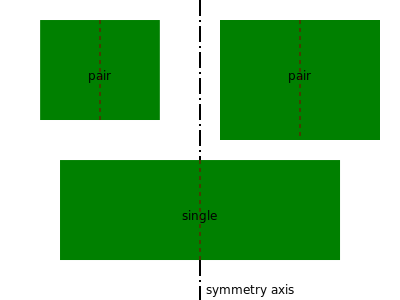
\includegraphics[height=84.6666687363mm, width=112.888891648mm]{FIG/constraint_symmetry.svg.pdf}}
  \put(206.0,-294.00002){\makebox(0,0)[l]{\smash{symmetry axis}}}
  \put(88.0,-80.0){\makebox(0,0)[l]{\smash{pair}}}
  \put(288.0,-80.0){\makebox(0,0)[l]{\smash{pair}}}
  \put(182.0,-220.0){\makebox(0,0)[l]{\smash{single}}}
\end{picture}
	\caption{horizontal symmetry constraint with one pair of modules and one single module}
	\label{fig:constraint_symmetry}
\end{figure}

\subsection{Alignment Constraint}
An alignment constraint defines a relative positions between modules, vertical or horizontal [\ref{fig:constraint_alignment}]. In the terminology of plantage you allways have a A- and B-module. In the case of a horizontal alignment the A-module is placed left of the B-module, in the other case of a vertical alignment the A-module is placed below of the B-module. Additionally it is possible to define a minimum distance between the modules.

\begin{figure}
	\centering
	\setlength{\unitlength}{0.282222229121mm}
\begin{picture}(400.0, 200.0)(0, -200.0)
  \put(0,-200.0){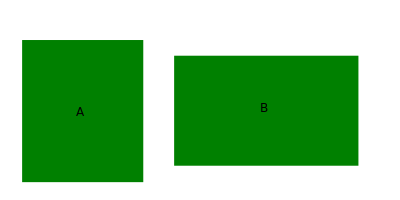
\includegraphics[height=56.4444458242mm, width=112.888891648mm]{FIG/constraint_alignment.svg.pdf}}
  \put(76.0,-116.0){\makebox(0,0)[l]{\smash{A}}}
  \put(260.0,-112.0){\makebox(0,0)[l]{\smash{B}}}
\end{picture}
	\caption{horizontal alignment constraint}
	\label{fig:constraint_alignment}
\end{figure}

\subsection{Group Symmetry Constraint}
The group symmetry constraint is nearly the same like the symmetry constraint. The only difference is, that it can be applied to groups instead of modules. Again we can have single groups, which are self symmetric placed, or pair groups, which are pairwise symmetric to the symmetry axis.

\subsection{Group Alignment Constraint}
Again the group alignment constraint is nearly the same like the alignment constraint with the only difference, that it can be applied to groups.

\subsection{Same Variants Constraint}
The same variants constraint is again very important to for example given differential pairs. To get as far as possible same characterisitics in one placement these modules should have the same variants. They can still have various different variants, but in one certain placement for these modules the same variant is selected.

\section{Technology Rules}
Typically the manufacturer of the chip provides a so called \textit{tech-file} for the circuit designer, which he can use to create the layout. This information includes for example the minimum distances between two modules. As the knowledge of the manufacturers is very important to them the technology-files are kept secret, and therefore no real standard for them exists. The following descriptions are based on a technology file from Austria Microsystems, which was available for this project. We assume, that other possible formats can be transformed through the ICFBInterface into something similar. The rules were already extract through a skill script from cadence, but they were not stored or looped through to plantage. The technology rules can have four different types:

\begin{itemize}
\item minimum width
\item minimum spacing
\item minimum notch
\item minimum enclosure
\end{itemize}

The first two rules, considering minimum width and spaces, have one value, the actual minimum width or distance, and the layer, which they should be applied on. The last two types have also a value, but additionally two layers, on which they must be considered. But let us first get to know the other two types.

PICTURE MISSING MINIMUM SPACING

The minimum spacing rule is quite easy to understand, it only describes a minimal distance between two shapes on a certain layer. These rules may not be considered if deep trench isolated transistors are concerned, but this doesn't affect the routing. Deep trench isolated transistors result only in a possible bigger, combined, forbidden area.

PICTURE MISSING MINIMUM WIDTH

Minimum widths are very central technology rules for the routing. These values are used as width for the routes and can be different for every layer.

PICTURE MISSING MINIMUM NOTCH

DESCRIPTION MISSING MINIMUM NOTCH

PICTURE MISSING MINIMUM ENCLOSURE

The minimum enclosure rules describe minimum distances, which need to be met between shapes on different layers. Typically in a technology file we only have minimum enclosure rules, where one of the considered layers is a via layer. A via layer is during manufacturing an additional layer, in which the connections between the different layers are created. For the routing these rules result in the dimensions of the vias on the layers, which are connected.

PICTURE MISSING VIA DIMENSIONS

Every via definition must have two minimum enclosure rules, one for every layer, which is connected through the via. Additionally we need on minimum width rule for the via layer, which describes the width of the acutal connection. From these three rules we then can calculate the dimensions of the via, which typically differ for the two layers.

\[\text{via dimension} = 2 \cdot \text{minimun enclosure} + \text{minimum via width}\]